\documentclass[border=4pt]{standalone}
\usepackage{lmodern}
\usepackage[T1]{fontenc}
\usepackage{tikz}
\usetikzlibrary{arrows.meta, positioning, calc}
\begin{document}
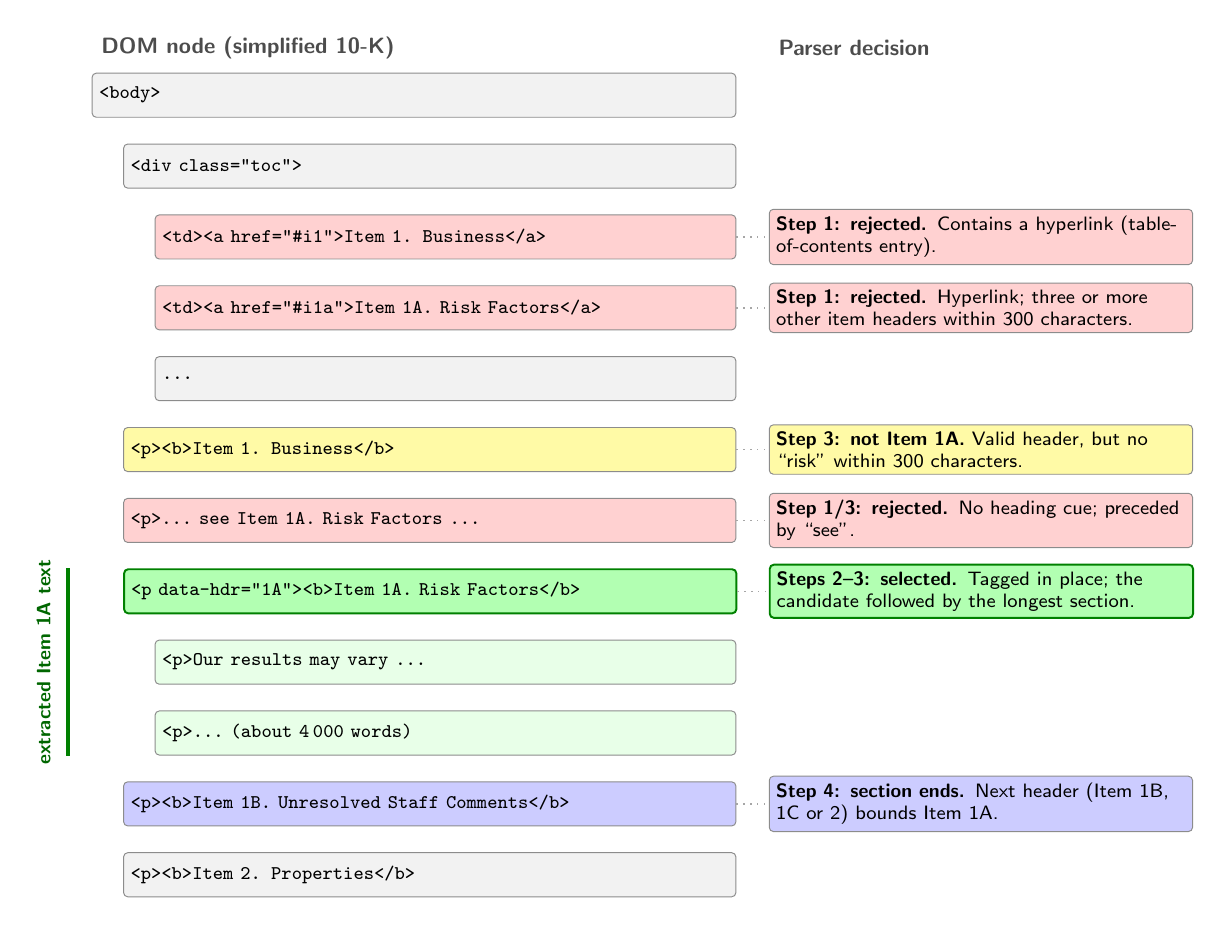
\begin{tikzpicture}[
    font=\sffamily\small,
    code/.style={rounded corners=1.5pt, draw=black!45, line width=0.35pt,
                 font=\ttfamily\scriptsize, align=left, anchor=west,
                 inner sep=2.5pt, minimum height=5.6mm},
    badge/.style={rounded corners=1.5pt, draw=black!45, line width=0.35pt,
                  font=\sffamily\scriptsize, align=left, anchor=west,
                  inner sep=2.5pt, text width=52mm, minimum height=5.6mm},
    link/.style={draw=black!35, dotted, line width=0.5pt},
    rej/.style={fill=red!18},
    part/.style={fill=yellow!35},
    sel/.style={fill=green!30, draw=green!50!black, line width=0.7pt},
    body/.style={fill=green!9},
    term/.style={fill=blue!20},
    neut/.style={fill=black!5},
]

% row(indent, y, style, name, text)
\newcommand{\row}[5]{%
  \node[code, #3, text width={80mm-#1}] (#4) at (#1,#2) {#5};}
% verdict(y, style, name, text, source row)
\newcommand{\verdict}[5]{%
  \node[badge, #2] (#3) at (86mm,#1) {#4};
  \draw[link] (#5.east) -- (#3.west);}

% ---- column headings ----
\node[anchor=west, font=\sffamily\bfseries\footnotesize, text=black!70]
  at (0,6mm) {DOM node (simplified 10-K)};
\node[anchor=west, font=\sffamily\bfseries\footnotesize, text=black!70]
  at (86mm,6mm) {Parser decision};

% ---- DOM rows ----
\row{0mm}{0mm}{neut}{r0}{<body>}
\row{4mm}{-9mm}{neut}{r1}{<div class="toc">}
\row{8mm}{-18mm}{rej}{r2}{<td><a href="\#i1">Item 1. Business</a>}
\row{8mm}{-27mm}{rej}{r3}{<td><a href="\#i1a">Item 1A. Risk Factors</a>}
\row{8mm}{-36mm}{neut}{r4}{\ldots}
\row{4mm}{-45mm}{part}{r5}{<p><b>Item 1. Business</b>}
\row{4mm}{-54mm}{rej}{r6}{<p>\ldots\ see Item 1A. Risk Factors \ldots}
\row{4mm}{-63mm}{sel}{r7}{<p data-hdr="1A"><b>Item 1A. Risk Factors</b>}
\row{8mm}{-72mm}{body}{r8}{<p>Our results may vary \ldots}
\row{8mm}{-81mm}{body}{r9}{<p>\ldots\ (about 4\,000 words)}
\row{4mm}{-90mm}{term}{r10}{<p><b>Item 1B. Unresolved Staff Comments</b>}
\row{4mm}{-99mm}{neut}{r11}{<p><b>Item 2. Properties</b>}

% ---- parser decisions ----
\verdict{-18mm}{rej}{v2}{\textbf{Step 1: rejected.} Contains a hyperlink
  (table-of-contents entry).}{r2}
\verdict{-27mm}{rej}{v3}{\textbf{Step 1: rejected.} Hyperlink; three or more
  other item headers within 300 characters.}{r3}
\verdict{-45mm}{part}{v5}{\textbf{Step 3: not Item 1A.} Valid header, but no
  ``risk'' within 300 characters.}{r5}
\verdict{-54mm}{rej}{v6}{\textbf{Step 1/3: rejected.} No heading cue; preceded
  by ``see''.}{r6}
\verdict{-63mm}{sel}{v7}{\textbf{Steps 2--3: selected.} Tagged in place; the
  candidate followed by the longest section.}{r7}
\verdict{-90mm}{term}{v10}{\textbf{Step 4: section ends.} Next header
  (Item 1B, 1C or 2) bounds Item 1A.}{r10}

% ---- extracted section bracket ----
\draw[green!50!black, line width=1.2pt]
  (-3mm,0 |- r7.north) -- (-3mm,0 |- r9.south);
\node[rotate=90, anchor=south, font=\sffamily\scriptsize\bfseries,
      text=green!40!black] at (-4mm,0 |- r8.west)
  {extracted Item 1A text};

\end{tikzpicture}
\end{document}
